\documentclass[10pt]{article}
\usepackage[margin=0.8in]{geometry}
\usepackage[utf8]{inputenc}
\usepackage[T1]{fontenc}
\usepackage{graphicx}
\usepackage[export]{adjustbox}
\usepackage{amsmath}
\usepackage{amsfonts}
\usepackage{amssymb}
\usepackage[version=4]{mhchem}
\usepackage{stmaryrd}
\usepackage{bbold}
\usepackage{fixltx2e}
\usepackage{caption}
\usepackage{mathtools}
\usepackage[parfill]{parskip}
\usepackage{float}
\usepackage{comment}


\begin{document}




\title{Lecture 18:  Dynamics (Lagrange Formulation)}
\date{Oct. 24, 2023}
\author{Wanxin Jin}
\maketitle

Compared to the previous (differential) kinematics concerning how a robot moves, robot dynamics in the following lectures concerns about why a robot moves. Dynamics equation establishes a relationship between the forces/torques and their acceleration/velocities/positions.

\section{Lagrange Mechanics}



Lagrange formulation provides a systematic way to derive  dynamics equation, independently of the reference coordinate frame. Once a set of \emph{independent} variables $q_{i}, i=1, \ldots, n$, termed generalized coordinates, are chosen which effectively describe an $n$-DOF robotic system, the Lagrangian of the  system can be defined as

$$
\mathcal{L}=\mathcal{T}-\mathcal{U}
$$

where $\mathcal{T}$ and $\mathcal{U}$ are the total kinetic energy and potential energy of the system, respectively. The dynamics equations from the Lagrangian is

$$
\frac{d}{d t} \frac{\partial \mathcal{L}}{\partial \dot{q}_{i}}-\frac{\partial \mathcal{L}}{\partial q_{i}}=\xi_{i} \quad i=1, \ldots, n
$$

where $\xi_{i}$ is the generalized force associated with  $q_{i}$ (the generalized force $\xi_i$ should be dual to $q_i$ in the sense that $\xi_i*q_i$ generate power). In compact form, the above equation can be written as 

$$
\frac{d}{d t}\left(\frac{\partial \mathcal{L}}{\partial \dot{\boldsymbol{q}}}\right)^{T}-\left(\frac{\partial \mathcal{L}}{\partial \boldsymbol{q}}\right)^{T}=\boldsymbol{\xi}
$$

For a manipulator with an open kinematic chain, the generalized coordinates are  joint variables $\boldsymbol{q}$. The  generalized forces are given by the net forces from  the joint actuator torques, the joint friction torques, as well as the joint torques induced by end-effector forces at the contact with the environment.





\section{Computation of Kinetic Energy}
Consider a manipulator with $n$  links. The total kinetic energy is due to the motion of each link and the motion of each joint actuator: 

$$
\mathcal{T}=\sum_{i=1}^{n}\left(\mathcal{T}_{\ell_{i}}+\mathcal{T}_{m_{i}}\right)
$$

where $\mathcal{T}_{\ell_{i}}$ is the kinetic energy of Link $i$ and $\mathcal{T}_{m_{i}}$ is the kinetic energy of the motor actuating Joint $i$

\subsection{Kinetic Energy of Link $i$}


\begin{figure}[H]
    \centering
    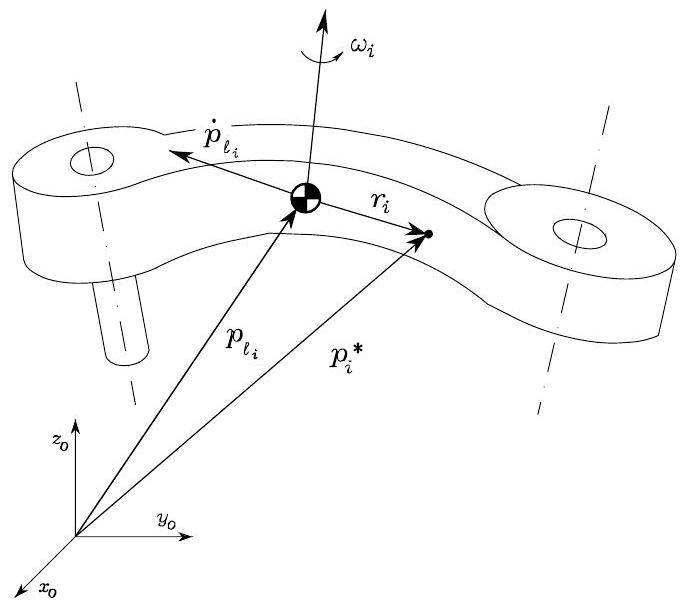
\includegraphics[max width=0.35\textwidth]{dynamics/linki_kinematics.jpg}
    \caption{Kinematic description of Link $i$ for Lagrange formulation}
    \label{fig:enter-label}
\end{figure}




The kinetic energy contribution of Link $i$ is given by

\begin{equation}\label{equ.link_ke}
            \mathcal{T}_{\ell_{i}}=\frac{1}{2} \int_{V_{\ell_{i}}} \dot{\boldsymbol{p}}_{i}^{* T} \dot{\boldsymbol{p}}_{i}^{*} \rho d V
\end{equation}

where $\dot{\boldsymbol{p}}_{i}^{*}$ denotes the linear velocity vector and $\rho$ is the density of the elementary particle of volume $d V ; V_{\ell_{i}}$ is the volume of Link $i$. Consider the position vector $\boldsymbol{p}_{i}^{*}$ of the elementary particle and the position vector $\boldsymbol{p}_{l_{i}}$ of the link center of mass, both expressed in the base frame. One has

$$
\boldsymbol{r}_{i}=\left[\begin{array}{lll}
r_{i x} & r_{i y} & r_{i z}
\end{array}\right]^{T}=\boldsymbol{p}_{i}^{*}-\boldsymbol{p}_{\ell_{i}}
$$

with

$$
\boldsymbol{p}_{\ell_{i}}=\frac{1}{m_{\ell_{i}}} \int_{V_{\ell_{i}}} \boldsymbol{p}_{i}^{*} \rho d V
$$





where $m_{\ell_{i}}$ is the link mass. As a consequence, the link point velocity can be expressed as

\begin{equation}\label{equ.2}
    \begin{aligned}
\dot{\boldsymbol{p}}_{i}^{*} & =\dot{\boldsymbol{p}}_{\ell_{i}}+\boldsymbol{\omega}_{i} \times \boldsymbol{r}_{i}  =\dot{\boldsymbol{p}}_{\ell_{i}}+\boldsymbol{S}\left(\boldsymbol{\omega}_{i}\right) \boldsymbol{r}_{i}
\end{aligned}
\end{equation}

where $\dot{\boldsymbol{p}}_{\ell_{i}}$ is the linear velocity of the center of mass and $\boldsymbol{\omega}_{i}$ is the angular velocity of the link. By substituting the velocity expression (\ref{equ.2}) into (\ref{equ.link_ke}), it leads to multiple terms

\textbf{Translational term}

$$
\frac{1}{2} \int_{V_{\ell_{i}}} \dot{\boldsymbol{p}}_{\ell_{i}}^{T} \dot{\boldsymbol{p}}_{\ell_{i}} \rho d V=\frac{1}{2} m_{\ell_{i}} \dot{\boldsymbol{p}}_{\ell_{i}}^{T} \dot{\boldsymbol{p}}_{\ell_{i}}
$$

\textbf{Cross term}

$$
2\left(\frac{1}{2} \int_{V_{\ell_{i}}} \dot{\boldsymbol{p}}_{\ell_{i}}^{T} \boldsymbol{S}\left(\boldsymbol{\omega}_{i}\right) \boldsymbol{r}_{i} \rho d V\right)=2\left(\frac{1}{2} \dot{\boldsymbol{p}}_{\ell_{i}}^{T} \boldsymbol{S}\left(\boldsymbol{\omega}_{i}\right) \int_{V_{\ell_{i}}}\left(\boldsymbol{p}_{i}^{*}-\boldsymbol{p}_{\ell_{i}}\right) \rho d V\right)=0
$$

\textbf{Rotational term}

$$
\frac{1}{2} \int_{V_{\ell_{i}}} \boldsymbol{r}_{i}^{T} \boldsymbol{S}^{T}\left(\boldsymbol{\omega}_{i}\right) \boldsymbol{S}\left(\boldsymbol{\omega}_{i}\right) \boldsymbol{r}_{i} \rho d V=\frac{1}{2} \boldsymbol{\omega}_{i}^{T}\left(\int_{V_{\ell_{i}}} \boldsymbol{S}^{T}\left(\boldsymbol{r}_{i}\right) \boldsymbol{S}\left(\boldsymbol{r}_{i}\right) \rho d V\right) \boldsymbol{\omega}_{i}=\frac{1}{2} \boldsymbol{\omega}_{i}^{T} \boldsymbol{I}_{\ell_{i}} \boldsymbol{\omega}_{i}
$$

In view of 

$$
\boldsymbol{S}\left(\boldsymbol{r}_{i}\right)=\left[\begin{array}{ccc}
0 & -r_{i z} & r_{i y} \\
r_{i z} & 0 & -r_{i x} \\
-r_{i y} & r_{i x} & 0
\end{array}\right]
$$


the matrix

$$
\begin{aligned}
\boldsymbol{I}_{\ell_{i}} & =\left[\begin{array}{ccc}
\int\left(r_{i y}^{2}+r_{i z}^{2}\right) \rho d V & -\int r_{i x} r_{i y} \rho d V & -\int r_{i x} r_{i z} \rho d V \\
* & \int\left(r_{i x}^{2}+r_{i z}^{2}\right) \rho d V & -\int r_{i y} r_{i z} \rho d V \\
* & * & \int\left(r_{i x}^{2}+r_{i y}^{2}\right) \rho d V
\end{array}\right] 
=  {\left[\begin{array}{ccc}
I_{\ell_{i} x x} & -I_{\ell_{i} x y} & -I_{\ell_{i} x z} \\
* & I_{\ell_{i} y y} & -I_{\ell_{i} y z} \\
* & * & I_{\ell_{i} z z}
\end{array}\right] . }
\end{aligned}
$$

represents the inertia tensor relative to the centre of mass of Link $i$ when expressed in the base frame. Notice that the inertia tensor, when expressed in the base frame, is configuration-dependent. If the angular velocity of Link $i$ is expressed with reference to a frame attached to the link (as in the Denavit-Hartenberg convention), it is

$$
\boldsymbol{\omega}_{i}^{i}=\boldsymbol{R}_{i}^{T} \boldsymbol{\omega}_{i}
$$

where $\boldsymbol{R}_{i}$ is the rotation matrix from Link $i$ frame to the base frame. When referred to the link frame, the inertia tensor is constant. Let $\boldsymbol{I}_{\ell_{i}}^{i}$ denote such tensor:

$$
\boldsymbol{I}_{\ell_{i}}^{i}=\boldsymbol{R}_{i}^{T} \boldsymbol{I}_{\ell_{i}} \boldsymbol{R}_{i}
$$

If the axes of Link $i$ frame coincide with the central axes of inertia, the inertia tensor relative to the centre of mass is a diagonal matrix. By summing the translational and rotational terms, 

$$
\mathcal{T}_{\ell_{i}}=\frac{1}{2} m_{\ell_{i}} \dot{\boldsymbol{p}}_{\ell_{i}}^{T} \dot{\boldsymbol{p}}_{\ell_{i}}+\frac{1}{2} \boldsymbol{\omega}_{i}^{T} \boldsymbol{R}_{i} \boldsymbol{I}_{\ell_{i}}^{i} \boldsymbol{R}_{i}^{T} \boldsymbol{\omega}_{i}
$$

At this point, it is necessary to express the kinetic energy as a function of the generalized coordinates of the system, that are the joint variables. To this end, 

$$
\begin{aligned}
\dot{\boldsymbol{p}}_{\ell_{i}} & =\boldsymbol{\jmath}_{P 1}^{\left(\ell_{i}\right)} \dot{q}_{1}+\ldots+\boldsymbol{J}_{P i}^{\left(\ell_{i}\right)} \dot{q}_{i}=\boldsymbol{J}_{P}^{\left(\ell_{i}\right)} \dot{\boldsymbol{q}} \\
\boldsymbol{\omega}_{i} & =\boldsymbol{\jmath}_{O 1}^{\left(\ell_{i}\right)} \dot{q}_{1}+\ldots+\boldsymbol{J}_{O i}^{\left(\ell_{i}\right)} \dot{q}_{i}=\boldsymbol{J}_{O}^{\left(\ell_{i}\right)} \dot{\boldsymbol{q}},
\end{aligned}
$$

where the contributions of the Jacobian columns relative to the joint velocities have been taken into account up to current Link $i$. The Jacobians to consider are then:

$$
\begin{aligned}
\boldsymbol{J}_{P}^{\left(\ell_{i}\right)}  =\left[\begin{array}{llllll}
\boldsymbol{J}_{P 1}^{\left(\ell_{i}\right)} & \ldots & \boldsymbol{J}_{P i}^{\left(\ell_{i}\right)} & \mathbf{0} & \ldots & \mathbf{0}
\end{array}\right]  \qquad
\boldsymbol{J}_{O}^{\left(\ell_{i}\right)}  =\left[\begin{array}{llllll}
\boldsymbol{J}_{O 1}^{\left(\ell_{i}\right)} & \ldots & \boldsymbol{J}_{O i}^{\left(\ell_{i}\right)} & \mathbf{0} & \ldots & \mathbf{0}
\end{array}\right] ;
\end{aligned}
$$ 

Here



$$
\begin{gathered}
\boldsymbol{J}_{P j}^{\left(\ell_{i}\right)}= \begin{cases}\boldsymbol{z}_{j-1} & \text { for a prismatic joint } \\
\boldsymbol{z}_{j-1} \times\left(\boldsymbol{p}_{\ell_{i}}-\boldsymbol{p}_{j-1}\right) &
\text { for a revolute joint }\end{cases} \qquad
\boldsymbol{\jmath}_{O j}^{\left(\ell_{i}\right)}= \begin{cases}\mathbf{0} & \text { for a prismatic joint } \\
\boldsymbol{z}_{j-1} & \text { for a revolute joint. }\end{cases}
\end{gathered}
$$

where $\boldsymbol{p}_{j-1}$ is the position  of the origin of Frame $j-1$ and $\boldsymbol{z}_{j-1}$ is the unit vector of axis $z$ of Frame $j-1$. 



It follows that the kinetic energy of Link $i$ can be written as

$$
\mathcal{T}_{\ell_{i}}=\frac{1}{2} m_{\ell_{i}} \dot{\boldsymbol{q}}^{T} \boldsymbol{J}_{P}^{\left(\ell_{i}\right) T} \boldsymbol{J}_{P}^{\left(\ell_{i}\right)} \dot{\boldsymbol{q}}+\frac{1}{2} \dot{\boldsymbol{q}}^{T} \boldsymbol{J}_{O}^{\left(\ell_{i}\right) T} \boldsymbol{R}_{i} \boldsymbol{I}_{\ell_{i}}^{i} \boldsymbol{R}_{i}^{T} \boldsymbol{J}_{O}^{\left(\ell_{i}\right)} \dot{\boldsymbol{q}}
$$

\subsection{Kinetic Energy of Motor $i$}


\begin{figure}[H]
    \centering
    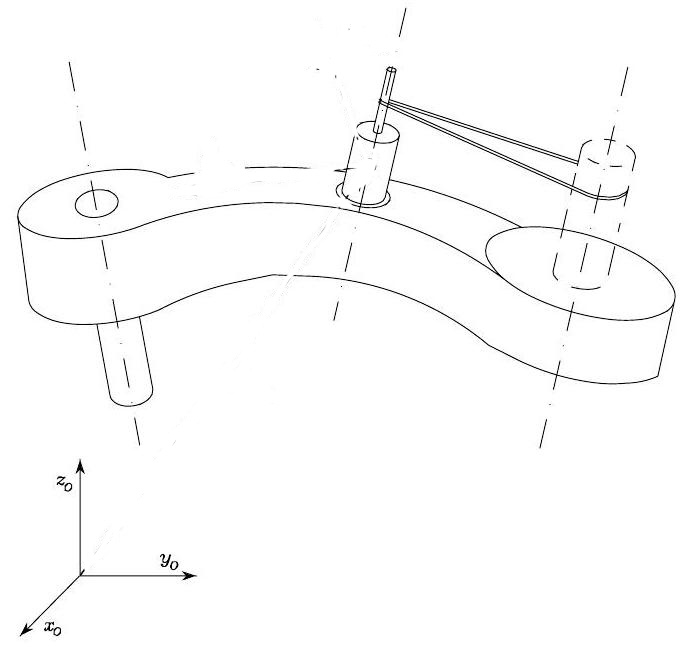
\includegraphics[max width=0.35\textwidth]{dynamics/motori_kinematics.jpg}
    \caption{Kinematic description of Motor $i$}
    \label{fig:enter-label}
\end{figure}




The motor of Joint $i$ is assumed to be located on Link $i-1$. The kinetic energy contribution of the motor of Joint $i$ can be computed in a formally analogous way to that of the link. Consider the typical case of rotary electric motors (that can actuate both revolute and prismatic joints by means of suitable transmissions). It can be assumed that the contribution of the fixed part (stator) is included in that of the link on which such motor is located, and thus the sole contribution of the rotor is to be computed.

The kinetic energy of Rotor $i$ can be written as

$$
\mathcal{T}_{m_{i}}=\frac{1}{2} m_{m_{i}} \dot{\boldsymbol{p}}_{m_{i}}^{T} \dot{\boldsymbol{p}}_{m_{i}}+\frac{1}{2} \boldsymbol{\omega}_{m_{i}}^{T} \boldsymbol{I}_{m_{i}} \boldsymbol{\omega}_{m_{i}}
$$

where $m_{m_{i}}$ is the mass of the rotor, $\dot{\boldsymbol{p}}_{m_{i}}$ denotes the linear velocity of the centre of mass of the rotor, $\boldsymbol{I}_{m_{i}}$ is the inertia tensor of the rotor relative to its centre of mass, and $\boldsymbol{\omega}_{m_{i}}$ denotes the angular velocity of the rotor.

Let $\vartheta_{m_{i}}$ denote the angular position of the rotor. On the assumption of a rigid transmission, one has

$$
k_{r i} \dot{q}_{i}=\dot{\vartheta}_{m_{i}}
$$

where $k_{r i}$ is  gear reduction ratio. For a prismatic joint,  gear reduction ratio is a dimensional quantity.

The total angular velocity of the rotor is

$$
\boldsymbol{\omega}_{m_{i}}=\boldsymbol{\omega}_{i-1}+k_{r i} \dot{q}_{i} \boldsymbol{z}_{m_{i}}
$$

where $\boldsymbol{\omega}_{i-1}$ is the angular velocity of Link $i-1$ on which the motor is located, and $\boldsymbol{z}_{m_{i}}$ denotes the unit vector along the rotor axis.

To express the rotor kinetic energy as a function of the joint variables, it is worth expressing the linear velocity of the rotor centre of mass as

$$
\dot{\boldsymbol{p}}_{m_{i}}=\boldsymbol{J}_{P}^{\left(m_{i}\right)} \dot{\boldsymbol{q}}
$$

The Jacobian to compute is then

$$
\boldsymbol{J}_{P}^{\left(m_{i}\right)}=\left[\begin{array}{llllll}
\boldsymbol{J}_{P 1}^{\left(m_{i}\right)} & \ldots & \boldsymbol{J}_{P, i-1}^{\left(m_{i}\right)} & \mathbf{0} & \ldots & \mathbf{0}
\end{array}\right]
$$

whose columns are given by

$$
\boldsymbol{J}_{P j}^{\left(m_{i}\right)}= \begin{cases}\boldsymbol{z}_{j-1} & \text { for a prismatic joint } \\ \boldsymbol{z}_{j-1} \times\left(\boldsymbol{p}_{m_{i}}-\boldsymbol{p}_{j-1}\right) & \text { for a revolute joint }\end{cases}
$$

where $\boldsymbol{p}_{j-1}$ is the position vector of the origin of Frame $j-1$. 

The angular velocity expressed as a function of the joint variables is
$$
\boldsymbol{\omega}_{m_{i}}=\boldsymbol{J}_{O}^{\left(m_{i}\right)} \dot{\boldsymbol{q}}
$$

The Jacobian to compute is then

$$
\boldsymbol{J}_{O}^{\left(m_{i}\right)}=\left[\begin{array}{llllll}
\boldsymbol{J}_{O 1}^{\left(m_{i}\right)} & \ldots & \boldsymbol{J}_{O, i}^{\left(m_{i}\right)} & \mathbf{0} & \ldots & \mathbf{0}
\end{array}\right]
$$

whose columns are

$$
\boldsymbol{\jmath}_{O j}^{\left(m_{i}\right)}= \begin{cases}\boldsymbol{J}_{O j}^{\left(\ell_{i}\right)} & j=1, \ldots, i-1 \\ k_{r i} \boldsymbol{z}_{m_{i}} & j=i .\end{cases}
$$



Hence, the kinetic energy of Rotor $i$ can be written as

$$
\mathcal{T}_{m_{i}}=\frac{1}{2} m_{m_{i}} \dot{\boldsymbol{q}}^{T} \boldsymbol{J}_{P}^{\left(m_{i}\right) T} \boldsymbol{J}_{P}^{\left(m_{i}\right)} \dot{\boldsymbol{q}}+\frac{1}{2} \dot{\boldsymbol{q}}^{T} \boldsymbol{J}_{O}^{\left(m_{i}\right) T} \boldsymbol{R}_{m_{i}} \boldsymbol{I}_{m_{i}}^{m_{i}} \boldsymbol{R}_{m_{i}}^{T} \boldsymbol{J}_{O}^{\left(m_{i}\right)} \dot{\boldsymbol{q}}
$$

\subsection{Total Kinetic Energy}

Finally, by summing the kinetic energies of Links and motors, the total kinetic energy of the manipulator with actuators is given by the quadratic form

$$
\mathcal{T}=\frac{1}{2} \dot{\boldsymbol{q}}^{T} \boldsymbol{B}(\boldsymbol{q}) \dot{\boldsymbol{q}}=\frac{1}{2} \sum_{i=1}^{n} \sum_{j=1}^{n} b_{i j}(\boldsymbol{q}) \dot{q}_{i} \dot{q}_{j}
$$

where

$$
\begin{aligned}
\boldsymbol{B}(\boldsymbol{q})=\sum_{i=1}^{n}\left(m_{\ell_{i}}\right. & \boldsymbol{J}_{P}^{\left(\ell_{i}\right) T} \boldsymbol{J}_{P}^{\left(\ell_{i}\right)}+\boldsymbol{J}_{O}^{\left(\ell_{i}\right) T} \boldsymbol{R}_{i} \boldsymbol{I}_{\ell_{i}}^{i} \boldsymbol{R}_{i}^{T} \boldsymbol{J}_{O}^{\left(\ell_{i}\right)}+\left.  m_{m_{i}} \boldsymbol{J}_{P}^{\left(m_{i}\right) T} \boldsymbol{J}_{P}^{\left(m_{i}\right)}+\boldsymbol{J}_{O}^{\left(m_{i}\right) T} \boldsymbol{R}_{m_{i}} \boldsymbol{I}_{m_{i}}^{m_{i}} \boldsymbol{R}_{m_{i}}^{T} \boldsymbol{J}_{O}^{\left(m_{i}\right)}\right)
\end{aligned}
$$

is the $(n \times n)$ inertia matrix which is  symmetric, positive definite, and configuration - dependent (in general).


\subsection{Computation of Potential Energy}
As done for kinetic energy, the potential energy stored in the manipulator is given by the sum of the contributions relative to each link as well as to each rotor:

$$
\mathcal{U}=\sum_{i=1}^{n}\left(\mathcal{U}_{\ell_{i}}+\mathcal{U}_{m_{i}}\right)
$$

On the assumption of rigid links, the potential energy of gravitational forces is

$$
\mathcal{U}_{\ell_{i}}=-\int_{V_{\ell_{i}}} \boldsymbol{g}_{0}^{T} \boldsymbol{p}_{i}^{*} \rho d V=-m_{\ell_{i}} \boldsymbol{g}_{0}^{T} \boldsymbol{p}_{\ell_{i}}
$$

where $\boldsymbol{g}_{0}$ is the gravity acceleration vector in the base frame (e.g., $\boldsymbol{g}_{0}=$ $\left[\begin{array}{lll}0 & 0 & -g\end{array}\right]^{T}$ if $z$ is the vertical axis), and $\boldsymbol{p}_{\ell_{i}}$ the center of mass of Link $i$. As regards the contribution of Rotor $i$, one has

$$
\mathcal{U}_{m_{i}}=-m_{m_{i}} \boldsymbol{g}_{0}^{T} \boldsymbol{p}_{m_{i}}
$$

The total potential energy is given by

$$
\mathcal{U}=-\sum_{i=1}^{n}\left(m_{\ell_{i}} \boldsymbol{g}_{0}^{T} \boldsymbol{p}_{\ell_{i}}+m_{m_{i}} \boldsymbol{g}_{0}^{T} \boldsymbol{p}_{m_{i}}\right)
$$

which reveals that potential energy, through the vectors $\boldsymbol{p}_{\ell_{i}}$ and $\boldsymbol{p}_{m_{i}}$ is a function only of the joint variables $\boldsymbol{q}$, and not of the joint velocities $\dot{\boldsymbol{q}}$

\subsection{Equations of Motion}
Having computed the total kinetic and potential energy of the system, the Lagrangian for the manipulator is

$$
\mathcal{L}(\boldsymbol{q}, \dot{\boldsymbol{q}})=\mathcal{T}(\boldsymbol{q}, \dot{\boldsymbol{q}})-\mathcal{U}(\boldsymbol{q})
$$

Taking the derivatives required by Lagrange equations $
\frac{d}{d t}\left(\frac{\partial \mathcal{L}}{\partial \dot{\boldsymbol{q}}}\right)^{T}-\left(\frac{\partial \mathcal{L}}{\partial \boldsymbol{q}}\right)^{T}=\boldsymbol{\xi}
$ and recalling that $\mathcal{U}$ does not depend on $\dot{\boldsymbol{q}}$ yields

$$
\boldsymbol{B}(\boldsymbol{q}) \ddot{\boldsymbol{q}}+\boldsymbol{n}(\boldsymbol{q}, \dot{\boldsymbol{q}})=\boldsymbol{\xi}
$$

where

$$
\boldsymbol{n}(\boldsymbol{q}, \dot{\boldsymbol{q}})=\dot{\boldsymbol{B}}(\boldsymbol{q}) \dot{\boldsymbol{q}}-\frac{1}{2}\left(\frac{\partial}{\partial \boldsymbol{q}}\left(\dot{\boldsymbol{q}}^{T} \boldsymbol{B}(\boldsymbol{q}) \dot{\boldsymbol{q}}\right)\right)^{T}+\left(\frac{\partial \mathcal{U}(\boldsymbol{q})}{\partial \boldsymbol{q}}\right)^{T}
$$

In detail, noticing that $\mathcal{U}$ does not depend on $\dot{\boldsymbol{q}}$ and 

$$
\begin{aligned}
\frac{d}{d t}\left(\frac{\partial \mathcal{L}}{\partial \dot{q}_{i}}\right)=\frac{d}{d t}\left(\frac{\partial \mathcal{T}}{\partial \dot{q}_{i}}\right) & =\sum_{j=1}^{n} b_{i j}(\boldsymbol{q}) \ddot{q}_{j}+\sum_{j=1}^{n} \frac{d b_{i j}(\boldsymbol{q})}{d t} \dot{q}_{j} =\sum_{j=1}^{n} b_{i j}(\boldsymbol{q}) \ddot{q}_{j}+\sum_{j=1}^{n} \sum_{k=1}^{n} \frac{\partial b_{i j}(\boldsymbol{q})}{\partial q_{k}} \dot{q}_{k} \dot{q}_{j}
\end{aligned}
$$

and

$$
\frac{\partial \mathcal{T}}{\partial q_{i}}=\frac{1}{2} \sum_{j=1}^{n} \sum_{k=1}^{n} \frac{\partial b_{j k}(\boldsymbol{q})}{\partial q_{i}} \dot{q}_{k} \dot{q}_{j}
$$

 Further,

$$
\begin{aligned}
\frac{\partial \mathcal{U}}{\partial q_{i}} & =-\sum_{j=1}^{n}\left(m_{\ell_{j}} \boldsymbol{g}_{0}^{T} \frac{\partial \boldsymbol{p}_{\ell_{j}}}{\partial q_{i}}+m_{m_{j}} \boldsymbol{g}_{0}^{T} \frac{\partial \boldsymbol{p}_{m_{j}}}{\partial q_{i}}\right) =-\sum_{j=1}^{n}\left(m_{\ell_{j}} \boldsymbol{g}_{0}^{T} \boldsymbol{J}_{P i}^{\left(\ell_{j}\right)}(\boldsymbol{q})+m_{m_{j}} \boldsymbol{g}_{0}^{T} \boldsymbol{J}_{P i}^{\left(m_{j}\right)}(\boldsymbol{q})\right)=g_{i}(\boldsymbol{q})
\end{aligned}
$$


As a result, the equations of motion are

$$
\sum_{j=1}^{n} b_{i j}(\boldsymbol{q}) \ddot{q}_{j}+\sum_{j=1}^{n} \sum_{k=1}^{n} h_{i j k}(\boldsymbol{q}) \dot{q}_{k} \dot{q}_{j}+g_{i}(\boldsymbol{q})=\xi_{i} \quad i=1, \ldots, n .
$$

where

$$
h_{i j k}=\frac{\partial b_{i j}}{\partial q_{k}}-\frac{1}{2} \frac{\partial b_{j k}}{\partial q_{i}}
$$

A physical interpretation of the above reveals that:

\begin{itemize}
  \item For the acceleration terms: 
  The coefficient $b_{i i}$ represents the moment of inertia at Joint $i$ axis, in the current manipulator configuration, when the other joints are blocked. The coefficient $b_{i j}$ accounts for the effect of acceleration of Joint $j$ on Joint $j$.

  \item For the quadratic velocity terms: The term $h_{i j j} \dot{q}_{j}^{2}$ is the centrifugal effect induced on Joint $i$ by velocity of Joint $j$. The term $h_{i j k} \dot{q}_{j} \dot{q}_{k}$ represents the Coriolis effect induced on Joint $i$ by velocities of Joints $j$ and $k$.

\item For the configuration-dependent terms:
The term $g_{i}$ represents the moment generated at Joint $i$ axis of the manipulator, in the current configuration, by the presence of gravity.

\end{itemize}








Regarding the generalized force $\boldsymbol{\xi}$ at the manipulator joints, it is
\begin{equation}
    \boldsymbol{\xi}=\underbrace{\boldsymbol{\tau}}_{\text{motor torque}}-\underbrace{\boldsymbol{F}_{v} \dot{\boldsymbol{q}}}_{\text{viscous friction torques}}-\underbrace{\boldsymbol{F}_{s} \operatorname{sgn}(\dot{\boldsymbol{q}})}_{\text{Coulomb friction torques}}-\underbrace{\boldsymbol{J}^{T}(\boldsymbol{q}) \boldsymbol{h}_{e}}_{\text{torques induced by  contact forces.}}
\end{equation}

where $\boldsymbol{F}_{v}$ denotes the $(n \times n)$ diagonal matrix of viscous friction coefficients; $\boldsymbol{F}_{s}$ is an $(n \times n)$ diagonal matrix and $\operatorname{sgn}(\dot{\boldsymbol{q}})$ denotes the $(n \times 1)$ vector whose components are given by the sign functions of the single joint velocities; and $\boldsymbol{h}_{e}$ denotes the vector of force and moment exerted by the end-effector on the environment.


In summary, the equations of motion for a robot manipulator is

$$
\boldsymbol{B}(\boldsymbol{q}) \ddot{\boldsymbol{q}}+\boldsymbol{C}(\boldsymbol{q}, \dot{\boldsymbol{q}}) \dot{\boldsymbol{q}}+\boldsymbol{F}_{v} \dot{\boldsymbol{q}}+\boldsymbol{F}_{s} \operatorname{sgn}(\dot{\boldsymbol{q}})+\boldsymbol{g}(\boldsymbol{q})=\boldsymbol{\tau}-\boldsymbol{J}^{T}(\boldsymbol{q}) \boldsymbol{h}_{e}
$$

where $\boldsymbol{C}$ is a suitable $(n \times n)$ matrix such that its elements $c_{i j}$ satisfy the equation

$$
\sum_{j=1}^{n} c_{i j} \dot{q}_{j}=\sum_{j=1}^{n} \Big(\sum_{k=1}^{n}c_{ijk}\dot{q}_{k}\Big) \dot{q}_{j}=\sum_{j=1}^{n} \sum_{k=1}^{n} h_{i j k} \dot{q}_{k} \dot{q}_{j}
$$

Here, the definition of $c_{ijk}$ is from
$$
\begin{aligned}
    \sum_{j=1}^{n} \sum_{k=1}^{n}h_{ijk}\dot{q}_{k} \dot{q}_{j}=
\sum_{j=1}^{n} \sum_{k=1}^{n}\Big(\frac{\partial b_{i j}}{\partial q_{k}}-\frac{1}{2} \frac{\partial b_{j k}}{\partial q_{i}}\Big)\dot{q}_{k} \dot{q}_{j}
&=\sum_{j=1}^{n} \sum_{k=1}^{n}\Big(\frac{1}{2}\frac{\partial b_{i j}}{\partial q_{k}}+\frac{1}{2}\frac{\partial b_{i j}}{\partial q_{k}}-\frac{1}{2} \frac{\partial b_{j k}}{\partial q_{i}}\Big)\dot{q}_{k} \dot{q}_{j}\\
&=\sum_{j=1}^{n} \sum_{k=1}^{n}\underbrace{\Big(\frac{1}{2}\frac{\partial b_{i j}}{\partial q_{k}}+\frac{1}{2}\frac{\partial b_{i k}}{\partial q_{j}}-\frac{1}{2} \frac{\partial b_{j k}}{\partial q_{i}}\Big)}_{c_{ijk}}\dot{q}_{k} \dot{q}_{j}
\end{aligned}
$$

Therefore, 
$$
c_{ijk}=\frac{1}{2}\Big(\frac{\partial b_{i j}}{\partial q_{k}}+\frac{\partial b_{i k}}{\partial q_{j}}- \frac{\partial b_{j k}}{\partial q_{i}}\Big)
$$

\subsection{Property of Dynamics Model: Skew-symmetry of $\dot{\boldsymbol{B}}-2\boldsymbol{C}$}

% \subsection{Property of Dynamic Model}
% \subsubsection{Skew-symmetry of Matrix $\dot{\boldsymbol{B}}-2\boldsymbol{C}$}

The proof idea: the total time derivative of kinetic energy of the manipulator equals the power generated by all the forces/torques including the gravity.

The time derivative of the kinetic energy:
\begin{equation}\label{equ.diff_kinenergy}
  \frac{d \mathcal{T}}{dt }=\frac{1}{2}\frac{d}{dt}\left(
    \dot{\boldsymbol{q}}^{T} \boldsymbol{B}(\boldsymbol{q})\dot{\boldsymbol{q}}
    \right)=\dot{\boldsymbol{q}}^{T}\boldsymbol{B}(\boldsymbol{q})\ddot{\boldsymbol{q}}+\frac{1}{2}\left(
    \dot{\boldsymbol{q}}^{T} \dot{\boldsymbol{B}}(\boldsymbol{q})\dot{\boldsymbol{q}}
    \right)
\end{equation}

The power generated by all (generalized) external forces including gravity:
\begin{equation}\label{equ.power_forces}
\dot{\boldsymbol{q}}^{T}(-\boldsymbol{F}_v{\dot{\boldsymbol{q}}}-\boldsymbol{F}_s\text{sgn}({\dot{\boldsymbol{q}}})-\boldsymbol{g}(\boldsymbol{q})-\boldsymbol{\tau}-\boldsymbol{J}^T(\boldsymbol{q})\boldsymbol{h}_{e})
\end{equation}

Let (\ref{equ.diff_kinenergy}) equal (\ref{equ.power_forces}), leading to 
\begin{equation}\label{equ.intermediate}
    \dot{\boldsymbol{q}}^{T}\boldsymbol{B}(\boldsymbol{q})\ddot{\boldsymbol{q}}+\frac{1}{2}\left(
    \dot{\boldsymbol{q}}^{T} \dot{\boldsymbol{B}}(\boldsymbol{q})\dot{\boldsymbol{q}}
    \right)=\dot{\boldsymbol{q}}^{T}(-\boldsymbol{F}_v{\dot{\boldsymbol{q}}}-\boldsymbol{F}_s\text{sgn}({\dot{\boldsymbol{q}}})-\boldsymbol{g}(\boldsymbol{q})-\boldsymbol{\tau}-\boldsymbol{J}^T(\boldsymbol{q})\boldsymbol{h}_{e})
\end{equation}
Recall the dynamics equation we have previously introduced,

$$
\boldsymbol{B}(\boldsymbol{q}) \ddot{\boldsymbol{q}}+\boldsymbol{C}(\boldsymbol{q}, \dot{\boldsymbol{q}}) \dot{\boldsymbol{q}}+\boldsymbol{F}_{v} \dot{\boldsymbol{q}}+\boldsymbol{F}_{s} \operatorname{sgn}(\dot{\boldsymbol{q}})+\boldsymbol{g}(\boldsymbol{q})=\boldsymbol{\tau}-\boldsymbol{J}^{T}(\boldsymbol{q}) \boldsymbol{h}_{e}
$$

We multiply $\dot{\boldsymbol{q}}^T$ on both sides of the above dynamics equation and subtract (\ref{equ.intermediate}) on both sides. This yields
\begin{equation}
  \frac{1}{2}  \dot{\boldsymbol{q}}^{T} \boldsymbol{B}(\boldsymbol{q})\dot{\boldsymbol{q}}-\dot{\boldsymbol{q}}^T\boldsymbol{C}(\boldsymbol{q}, \dot{\boldsymbol{q}}) \dot{\boldsymbol{q}}=\frac{1}{2}  \dot{\boldsymbol{q}}^{T} \left\big( \boldsymbol{B}(\boldsymbol{q})\dot{\boldsymbol{q}}-2\boldsymbol{C}(\boldsymbol{q}, \dot{\boldsymbol{q}})\right\big) \dot{\boldsymbol{q}}=\boldsymbol{0}
\end{equation}
which holds for any $\dot{\boldsymbol{q}}$. It means that
$\boldsymbol{B}(\boldsymbol{q})\dot{\boldsymbol{q}}-2\boldsymbol{C}(\boldsymbol{q}, \dot{\boldsymbol{q}})$
is a skew-symmetric matrix.

\begin{comment}

\subsubsection{Linearity in the Dynamic Parameters (Optional)}
An important property of the dynamic model is the linearity with respect to the dynamic parameters characterizing the manipulator links and rotors. By considering the union of Link $i$ and Rotor $i+1$ (augmented Link $i$ ), the kinetic energy contribution is given by

$$
\mathcal{T}_{i}=\mathcal{T}_{\ell_{i}}+\mathcal{T}_{m_{i+1}}
$$

where

$$
\mathcal{T}_{\ell_{i}}=\frac{1}{2} m_{\ell i} \dot{\boldsymbol{p}}_{\ell_{i}}^{T} \dot{\boldsymbol{p}}_{\ell_{i}}+\frac{1}{2} \boldsymbol{\omega}_{i}^{T} \boldsymbol{I}_{\ell_{i}} \boldsymbol{\omega}_{i}
$$

and

$$
\mathcal{T}_{m_{i+1}}=\frac{1}{2} m_{m_{i+1}} \dot{\boldsymbol{p}}_{m_{i+1}}^{T} \dot{\boldsymbol{p}}_{m_{i+1}}+\frac{1}{2} \boldsymbol{\omega}_{m_{i+1}}^{T} \boldsymbol{I}_{m_{i+1}} \boldsymbol{\omega}_{m_{i+1}}
$$

W.r.t. the center of mass of the augmented link, the linear velocities of the link and rotor can be expressed as

$$
\begin{aligned}
\dot{\boldsymbol{p}}_{\ell_{i}} & =\dot{\boldsymbol{p}}_{C_{i}}+\boldsymbol{\omega}_{i} \times \boldsymbol{r}_{C_{i}, \ell_{i}} \\
\dot{\boldsymbol{p}}_{m_{i+1}} & =\dot{\boldsymbol{p}}_{C_{i}}+\boldsymbol{\omega}_{i} \times \boldsymbol{r}_{C_{i}, m_{i+1}}
\end{aligned}
$$

with

$$
\begin{aligned}
\boldsymbol{r}_{C_{i}, \ell_{i}} & =\boldsymbol{p}_{\ell_{i}}-\boldsymbol{p}_{C_{i}} \\
\boldsymbol{r}_{C_{i}, m_{i+1}} & =\boldsymbol{p}_{m_{i+1}}-\boldsymbol{p}_{C_{i}},
\end{aligned}
$$

where $\boldsymbol{p}_{C_{i}}$ denotes the position vector of the centre of mass of augmented Link $i$.

    Substituting $\boldsymbol{r}_{C_{i}, \ell_{i}}  =\boldsymbol{p}_{\ell_{i}}-\boldsymbol{p}_{C_{i}}$ to the kinetic energy of the link gives

$$
\begin{aligned}
\mathcal{T}_{\ell_{i}}= & \frac{1}{2} m_{\ell i} \dot{\boldsymbol{p}}_{C_{i}}^{T} \dot{\boldsymbol{p}}_{C_{i}}+\dot{\boldsymbol{p}}_{C_{i}}^{T} \boldsymbol{S}\left(\boldsymbol{\omega}_{i}\right) m_{\ell_{i}} \boldsymbol{r}_{C_{i}, \ell_{i}}  +\frac{1}{2} m_{\ell_{i}} \boldsymbol{\omega}_{i}^{T} \boldsymbol{S}^{T}\left(\boldsymbol{r}_{C_{i}, \ell_{i}}\right) \boldsymbol{S}\left(\boldsymbol{r}_{C_{i}, \ell_{i}}\right) \boldsymbol{\omega}_{i}+\frac{1}{2} \boldsymbol{\omega}_{i}^{T} \boldsymbol{I}_{\ell_{i}} \boldsymbol{\omega}_{i} .
\end{aligned}
$$

By virtue of Steiner theorem, the matrix

$$
\overline{\boldsymbol{I}}_{\ell_{i}}=\boldsymbol{I}_{\ell_{i}}+m_{\ell_{i}} \boldsymbol{S}^{T}\left(\boldsymbol{r}_{C_{i}, \ell_{i}}\right) \boldsymbol{S}\left(\boldsymbol{r}_{C_{i}, \ell_{i}}\right)
$$

represents the inertia tensor relative to the overall centre of mass $\boldsymbol{p}_{C_{i}}$, which contains an additional contribution due to the translation of the pole with respect to which the tensor is evaluated. Therefore, 

$$
\mathcal{T}_{\ell_{i}}=\frac{1}{2} m_{\ell i} \dot{\boldsymbol{p}}_{C_{i}}^{T} \dot{\boldsymbol{p}}_{C_{i}}+\dot{\boldsymbol{p}}_{C_{i}}^{T} \boldsymbol{S}\left(\boldsymbol{\omega}_{i}\right) m_{\ell_{i}} \boldsymbol{r}_{C_{i}, \ell_{i}}+\frac{1}{2} \boldsymbol{\omega}_{i}^{T} \overline{\boldsymbol{I}}_{\ell_{i}} \boldsymbol{\omega}_{i}
$$

In a similar fashion, substituting $\boldsymbol{r}_{C_{i}, m_{i+1}}  =\boldsymbol{p}_{m_{i+1}}-\boldsymbol{p}_{C_{i}}$ to the kinetic energy of the rotor gives

$$
\begin{gathered}
\mathcal{T}_{m_{i+1}}=\frac{1}{2} m_{m_{i+1}} \dot{\boldsymbol{p}}_{C_{i}}^{T} \dot{\boldsymbol{p}}_{C_{i}}+\dot{\boldsymbol{p}}_{C_{i}}^{T} \boldsymbol{S}\left(\boldsymbol{\omega}_{i}\right) m_{m_{i+1}} \boldsymbol{r}_{C_{i}, m_{i+1}}+\frac{1}{2} \boldsymbol{\omega}_{i}^{T} \overline{\boldsymbol{I}}_{m_{i+1}} \boldsymbol{\omega}_{i} \\
+k_{r, i+1} \dot{q}_{i+1} \boldsymbol{z}_{m_{i+1}}^{T} \boldsymbol{I}_{m_{i+1}} \boldsymbol{\omega}_{i}+\frac{1}{2} k_{r, i+1}^{2} \dot{q}_{i+1}^{2} \boldsymbol{z}_{m_{i+1}}^{T} \boldsymbol{I}_{m_{i+1}} \boldsymbol{z}_{m_{i+1}}
\end{gathered}
$$

where

$$
\overline{\boldsymbol{I}}_{m_{i+1}}=\boldsymbol{I}_{m_{i+1}}+m_{m_{i+1}} \boldsymbol{S}^{T}\left(\boldsymbol{r}_{C_{i}, m_{i+1}}\right) \boldsymbol{S}\left(\boldsymbol{r}_{C_{i}, m_{i+1}}\right) .
$$

Summing the kinetic energy of link and rotor gives the  kinetic energy of augmented Link $i$ 

$$
\begin{gathered}
\mathcal{T}_{i}=\frac{1}{2} m_{i} \dot{\boldsymbol{p}}_{C_{i}}^{T} \dot{\boldsymbol{p}}_{C_{i}}+\frac{1}{2} \boldsymbol{\omega}_{i}^{T} \overline{\boldsymbol{I}}_{i} \boldsymbol{\omega}_{i}+k_{r, i+1} \dot{q}_{i+1} \boldsymbol{z}_{m_{i+1}^{T}}^{T} \boldsymbol{I}_{m_{i+1}} \boldsymbol{\omega}_{i} +\frac{1}{2} k_{r, i+1}^{2} \dot{q}_{i+1}^{2} \boldsymbol{z}_{m_{i+1}}^{T} \boldsymbol{I}_{m_{i+1}} \boldsymbol{z}_{m_{i+1}},
\end{gathered}
$$

where $m_{i}=m_{\ell_{i}}+m_{m_{i+1}}$ and $\overline{\boldsymbol{I}}_{i}=\overline{\boldsymbol{I}}_{\ell_{i}}+\overline{\boldsymbol{I}}_{m_{i+1}}$ are respectively the overall mass and inertia tensor. 
Notice that the first two terms on the right-hand side  represent the kinetic energy contribution of the rotor when this is still, whereas the remaining two terms account for the rotor's own motion.

On the assumption that the rotor has a symmetric mass distribution about its axis of rotation, its inertia tensor expressed in a frame $\boldsymbol{R}_{m_{i}}$ with origin at the center of mass and axis $z_{m_{i}}$ aligned with the rotation axis is

$$
\boldsymbol{I}_{m_{i}}^{m_{i}}=\left[\begin{array}{ccc}
I_{m_{i} x x} & 0 & 0 \\
0 & I_{m_{i} y y} & 0 \\
0 & 0 & I_{m_{i} z z}
\end{array}\right]
$$

where $I_{m_{i} y y}=I_{m_{i} x x}$. As a consequence, the inertia tensor is invariant with respect to any rotation about axis $z_{m_{i}}$ and is, anyhow, constant when referred to any frame attached to Link $i-1$.

It is worth referring the inertia tensor of the link $\boldsymbol{I}_{i}$ to frame $\boldsymbol{R}_{i}$ attached to the link and the inertia tensor $\boldsymbol{I}_{m_{i+1}}$ to frame $\boldsymbol{R}_{m_{i+1}}$ so that it is diagonal. Thus,

$$
\boldsymbol{I}_{m_{i+1}} \boldsymbol{z}_{m_{i+1}}=\boldsymbol{R}_{m_{i+1}} \boldsymbol{I}_{m_{i+1}}^{m_{i+1}} \boldsymbol{R}_{m_{i+1}}^{T} \boldsymbol{z}_{m_{i+1}}=I_{m_{i+1}} \boldsymbol{z}_{m_{i+1}}
$$

where $I_{m_{i+1}}=I_{m_{i+1} z z}$ denotes the constant scalar moment of inertia of the rotor about its rotation axis

and

$$
\begin{aligned}
& \mathcal{T}_{i}=\frac{1}{2} m_{i} \dot{\boldsymbol{p}}_{C_{i}}^{i T} \dot{\boldsymbol{p}}_{C_{i}}^{i}+\frac{1}{2} \boldsymbol{\omega}_{i}^{i T} \overline{\boldsymbol{I}}_{i}^{i} \boldsymbol{\omega}_{i}^{i}+k_{r, i+1} \dot{q}_{i+1} I_{m_{i+1}} \boldsymbol{z}_{m_{i+1}}^{i T} \boldsymbol{\omega}_{i}^{i} +\frac{1}{2} k_{r, i+1}^{2} \dot{q}_{i+1}^{2} I_{m_{i+1}} .
\end{aligned}
$$

According to 

$$
\dot{\boldsymbol{p}}_{C_{i}}^{i}=\dot{\boldsymbol{p}}_{i}^{i}+\boldsymbol{\omega}_{i}^{i} \times \boldsymbol{r}_{i, C_{i}}^{i},
$$

where all the vectors have been referred to Frame $i$; note that $\boldsymbol{r}_{i, C_{i}}^{i}$ is fixed in such a frame, thus

$$
\begin{aligned}
\mathcal{T}_{i}=\frac{1}{2} m_{i} \dot{\boldsymbol{p}}_{i}^{i T} \dot{\boldsymbol{p}}_{i}^{i}+\dot{\boldsymbol{p}}_{i}^{i T} \boldsymbol{S}\left(\boldsymbol{\omega}_{i}^{i}\right) m_{i} \boldsymbol{r}_{i, C_{i}}^{i}+\frac{1}{2} \boldsymbol{\omega}_{i}^{i T} \widehat{\boldsymbol{I}}_{i}^{i} \boldsymbol{\omega}_{i}^{i}
+k_{r, i+1} \dot{q}_{i+1} I_{m_{i+1}} \boldsymbol{z}_{m_{i+1}}^{i T} \boldsymbol{\omega}_{i}^{i}+\frac{1}{2} k_{r, i+1}^{2} \dot{q}_{i+1}^{2} I_{m_{i+1}}
\end{aligned}
$$

where

$$
\widehat{\boldsymbol{I}}_{i}^{i}=\overline{\boldsymbol{I}}_{i}^{i}+m_{i} \boldsymbol{S}^{T}\left(\boldsymbol{r}_{i, C_{i}}^{i}\right) \boldsymbol{S}\left(\boldsymbol{r}_{i, C_{i}}^{i}\right)
$$

represents the inertia tensor with respect to the origin of Frame $i$ according to Steiner theorem

Let $\boldsymbol{r}_{i, C_{i}}^{i}=\left[\begin{array}{lll}\ell_{C_{i} x} & \ell_{C_{i} y} & \ell_{C_{i} z}\end{array}\right]^{T}$. The first moment of inertia is

$$
m_{i} \boldsymbol{r}_{i, C_{i}}^{i}=\left[\begin{array}{c}
m_{i} \ell_{C_{i} x} \\
m_{i} \ell_{C_{i} y} \\
m_{i} \ell_{C_{i} z}
\end{array}\right] .
$$

The inertia tensor of augmented Link $i$ is

$$
\begin{aligned}
& \widehat{\boldsymbol{I}}_{i}^{i}=\left[\begin{array}{ccc}
\bar{I}_{i x x}+m_{i}\left(\ell_{C_{i} y}^{2}+\ell_{C_{i} z}^{2}\right) & -\bar{I}_{i x y}-m_{i} \ell_{C_{i} x} \ell_{C_{i} y} & -\bar{I}_{i x z}-m_{i} \ell_{C_{i} x} \ell_{C_{i} z} \\
* & \bar{I}_{i y y}+m_{i}\left(\ell_{C_{i} x}^{2}+\ell_{C_{i} z}^{2}\right) & -\bar{I}_{i y z}-m_{i} \ell_{C_{i} y} \ell_{C_{i} z} \\
* & * & \bar{I}_{i z z}+m_{i}\left(\ell_{C_{i} x}^{2}+\ell_{C_{i} y}^{2}\right)
\end{array}\right] =\left[\begin{array}{ccc}
\widehat{I}_{i x x} & -\widehat{I}_{i x y} & -\widehat{I}_{i x z} \\
* & \widehat{I}_{i y y} & -\widehat{I}_{i y z} \\
* & * & \widehat{I}_{i z z}
\end{array}\right]
\end{aligned}
$$

Therefore, the kinetic energy of the augmented link is linear with respect to the dynamic parameters, namely, the mass, the three components of the first moment of inertia, the six components of the inertia tensor, and the moment of inertia of the rotor. As regards potential energy, 

$$
\mathcal{U}_{i}=-m_{i} \boldsymbol{g}_{0}^{i T} \boldsymbol{p}_{C_{i}}^{i}
$$

where the vectors have been referred to Frame $i$. According to the relation

$$
\boldsymbol{p}_{C_{i}}^{i}=\boldsymbol{p}_{i}^{i}+\boldsymbol{r}_{i, C_{i}}^{i}
$$


Thus,

$$
\mathcal{U}_{i}=-\boldsymbol{g}_{0}^{i T}\left(m_{i} \boldsymbol{p}_{i}^{i}+m_{i} \boldsymbol{r}_{i, C_{i}}^{i}\right)
$$

that is, the potential energy of the augmented link is linear with respect to the mass and the three components of the first moment of inertia. By summing the contributions of kinetic energy and potential energy for all augmented links, the Lagrangian of the system  can be expressed in the form

$$
\mathcal{L}=\sum_{i=1}^{n}\left(\boldsymbol{\beta}_{\mathcal{T} i}^{T}-\boldsymbol{\beta}_{\mathcal{U} i}^{T}\right) \boldsymbol{\pi}_{i}
$$

where $\boldsymbol{\pi}_{i}$ is the $(11 \times 1)$ vector of dynamic parameters, in which the moment of inertia of Rotor $i$ has been associated with the parameters of Link $i$ so as to simplify the notation.

In the above, $\boldsymbol{\beta}_{\mathcal{T} i}$ and $\boldsymbol{\beta}_{\mathcal{U} i}$ are two $(11 \times 1)$ vectors that allow the Lagrangian to be written as a function of $\boldsymbol{\pi}_{i}$. Such vectors are a function of the generalized coordinates of the mechanical system (and also of their derivatives as regards $\boldsymbol{\beta}_{\mathcal{T} i}$ ). In particular, it can be shown that $\boldsymbol{\beta}_{\mathcal{T} i}=$ $\boldsymbol{\beta}_{\mathcal{T} i}\left(q_{1}, q_{2}, \ldots, q_{i}, \dot{q}_{1}, \dot{q}_{2}, \ldots, \dot{q}_{i}\right)$ and $\boldsymbol{\beta}_{\mathcal{U} i}=\boldsymbol{\beta}_{\mathcal{U} i}\left(q_{1}, q_{2}, \ldots, q_{i}\right)$, i.e., they do not depend on the variables of the joints subsequent to Link $i$.

At this point, it should be observed how the derivations required by the Lagrange equations  do not alter the property of linearity in the parameters, and then the generalized force at Joint $i$ can be written as

$$
\xi_{i}=\sum_{j=1}^{n} \boldsymbol{y}_{i j}^{T} \boldsymbol{\pi}_{j}
$$

where

$$
\boldsymbol{y}_{i j}=\frac{d}{d t} \frac{\partial \boldsymbol{\beta}_{\mathcal{T}_{j}}}{\partial \dot{q}_{i}}-\frac{\partial \boldsymbol{\beta}_{\mathcal{T}_{j}}}{\partial q_{i}}+\frac{\partial \boldsymbol{\beta}_{\mathcal{U}_{j}}}{\partial q_{i}}
$$

Since the partial derivatives of $\boldsymbol{\beta}_{\mathcal{T} j}$ and $\boldsymbol{\beta}_{\mathcal{U} j}$  vanish for $j<i$, the following notable result is obtained:

$$
\left[\begin{array}{c}
\xi_{1} \\
\xi_{2} \\
\vdots \\
\xi_{n}
\end{array}\right]=\left[\begin{array}{cccc}
\boldsymbol{y}_{11}^{T} & \boldsymbol{y}_{12}^{T} & \ldots & \boldsymbol{y}_{1 n}^{T} \\
\mathbf{0}^{T} & \boldsymbol{y}_{22}^{T} & \ldots & \boldsymbol{y}_{2 n}^{T} \\
\vdots & \vdots & \ddots & \vdots \\
\mathbf{0}^{T} & \mathbf{0}^{T} & \ldots & \boldsymbol{y}_{n n}^{T}
\end{array}\right]\left[\begin{array}{c}
\boldsymbol{\pi}_{1} \\
\boldsymbol{\pi}_{2} \\
\vdots \\
\boldsymbol{\pi}_{n}
\end{array}\right]
$$

which yields the property of linearity of the model of a manipulator with respect to its dynamic parameters. Compactly, the above can be  written as

$$
\boldsymbol{\tau}=\boldsymbol{Y}(\boldsymbol{q}, \dot{\boldsymbol{q}}, \ddot{\boldsymbol{q}}) \boldsymbol{\pi}
$$
where $\boldsymbol{\pi}$ is a $(p \times 1)$ vector of constant parameters and $\boldsymbol{Y}$ is an $(n \times p)$ matrix which is a function of joint positions, velocities and accelerations; this matrix is usually called regressor. 

\end{comment}

\subsection{Examples: Two-link Planar Arm}



Consider the two-link planar arm below.

\begin{figure}[H]
    \centering
    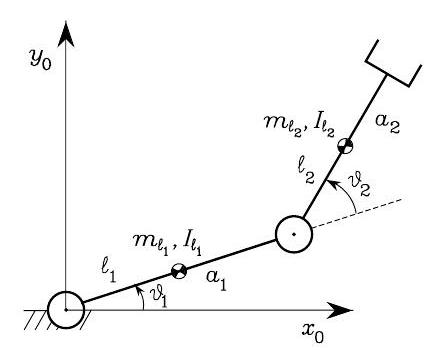
\includegraphics[max width=0.3\textwidth]{dynamics/2link_arm.jpg}
    \caption{Two-link planar arm}
    \label{fig:enter-label}
\end{figure}


The vector of generalized coordinates is $\boldsymbol{q}=\left[\begin{array}{ll}\vartheta_{1} & \vartheta_{2}\end{array}\right]^{T}$. Let $\ell_{1}, \ell_{2}$ be the distances of the centres of mass of the two links from the respective joint axes. Also let $m_{\ell_{1}}, m_{\ell_{2}}$ be the masses of the two links, and $m_{m_{1}}, m_{m_{2}}$ the masses of the rotors of the two joint motors. Finally, let $I_{m_{1}}, I_{m_{2}}$ be the moments of inertia with respect to the axes of the two rotors, and $I_{\ell_{1}}, I_{\ell_{2}}$ the moments of inertia relative to the
Centers of mass of the two links, respectively. It is assumed that $\boldsymbol{p}_{m_{i}}=\boldsymbol{p}_{i-1}$ and $\boldsymbol{z}_{m_{i}}=\boldsymbol{z}_{i-1}$, for $i=1,2$, i.e., the motors are located on the joint axes with centres of mass located at the origins of the respective frames.

With the chosen coordinate frames, computation of the Jacobians for each link is

$$
\boldsymbol{J}_{P}^{\left(\ell_{1}\right)}=\left[\begin{array}{cc}
-\ell_{1} s_{1} & 0 \\
\ell_{1} c_{1} & 0 \\
0 & 0
\end{array}\right] \quad J_{P}^{\left(\ell_{2}\right)}=\left[\begin{array}{cc}
-a_{1} s_{1}-\ell_{2} s_{12} & -\ell_{2} s_{12} \\
a_{1} c_{1}+\ell_{2} c_{12} & \ell_{2} c_{12} \\
0 & 0
\end{array}\right]
\quad
\boldsymbol{J}_{O}^{\left(\ell_{1}\right)}=\left[\begin{array}{ll}
0 & 0 \\
0 & 0 \\
1 & 0
\end{array}\right] \quad J_{O}^{\left(\ell_{2}\right)}=\left[\begin{array}{ll}
0 & 0 \\
0 & 0 \\
1 & 1
\end{array}\right]
$$

Notice that $\boldsymbol{\omega}_{i}$, for $i=1,2$, is aligned with $z_{0}$, and thus $\boldsymbol{R}_{i}$ has no effect. It is then possible to refer to the scalar moments of inertia $I_{\ell_{i}}$.

Computation of the Jacobians for each motor is

$$
\boldsymbol{J}_{P}^{\left(m_{1}\right)}=\left[\begin{array}{cc}
0 & 0 \\
0 & 0 \\
0 & 0
\end{array}\right] \quad \boldsymbol{J}_{P}^{\left(m_{2}\right)}=\left[\begin{array}{cc}
-a_{1} s_{1} & 0 \\
a_{1} c_{1} & 0 \\
0 & 0
\end{array}\right]\quad
\boldsymbol{J}_{O}^{\left(m_{1}\right)}=\left[\begin{array}{cc}
0 & 0 \\
0 & 0 \\
k_{r 1} & 0
\end{array}\right] \quad \boldsymbol{J}_{O}^{\left(m_{2}\right)}=\left[\begin{array}{cc}
0 & 0 \\
0 & 0 \\
1 & k_{r 2}
\end{array}\right]
$$



where $k_{r i}$ is the gear reduction ratio of Motor $i$.

The inertia matrix is

$$
\boldsymbol{B}(\boldsymbol{q})=\left[\begin{array}{cc}
b_{11}\left(\vartheta_{2}\right) & b_{12}\left(\vartheta_{2}\right) \\
b_{21}\left(\vartheta_{2}\right) & b_{22}
\end{array}\right]
$$

$$
\begin{aligned}
b_{11}= & I_{\ell_{1}}+m_{\ell_{1}} \ell_{1}^{2}+k_{r 1}^{2} I_{m_{1}}+I_{\ell_{2}}+m_{\ell_{2}}\left(a_{1}^{2}+\ell_{2}^{2}+2 a_{1} \ell_{2} c_{2}\right) \\
& \quad+I_{m_{2}}+m_{m_{2}} a_{1}^{2} \\
b_{12}= & b_{21}=I_{\ell_{2}}+m_{\ell_{2}}\left(\ell_{2}^{2}+a_{1} \ell_{2} c_{2}\right)+k_{r 2} I_{m_{2}} \\
b_{22}= & I_{\ell_{2}}+m_{\ell_{2}} \ell_{2}^{2}+k_{r 2}^{2} I_{m_{2}} .
\end{aligned}
$$

Compared to the previous example, the inertia matrix is now configurationdependent. Notice that the term $k_{r 2} I_{m_{2}}$ in the off-diagonal term of the inertia matrix derives from having considered the rotational part of the motor kinetic energy as due to the total angular velocity, i.e., its own angular velocity and that of the preceding link in the kinematic chain. At first approximation, especially in the case of high values of the gear reduction ratio, this contribution could be neglected; in the resulting reduced model, motor inertias would appear uniquely in the elements on the diagonal of the inertia matrix with terms of the type $k_{r i}^{2} I_{m_{i}}$

The computation of Christoffel symbols gives

$$
\begin{aligned}
& c_{111}=\frac{1}{2} \frac{\partial b_{11}}{\partial q_{1}}=0 \\
& c_{112}=c_{121}=\frac{1}{2} \frac{\partial b_{11}}{\partial q_{2}}=-m_{\ell_{2}} a_{1} \ell_{2} s_{2}=h \\
& c_{122}=\frac{\partial b_{12}}{\partial q_{2}}-\frac{1}{2} \frac{\partial b_{22}}{\partial q_{1}}=h \\
& c_{211}=\frac{\partial b_{21}}{\partial q_{1}}-\frac{1}{2} \frac{\partial b_{11}}{\partial q_{2}}=-h \\
& c_{212}=c_{221}=\frac{1}{2} \frac{\partial b_{22}}{\partial q_{1}}=0 \\
& c_{222}=\frac{1}{2} \frac{\partial b_{22}}{\partial q_{2}}=0
\end{aligned}
$$

leading to the matrix

$$
\boldsymbol{C}(\boldsymbol{q}, \dot{\boldsymbol{q}})=\left[\begin{array}{cc}
h \dot{\vartheta}_{2} & h\left(\dot{\vartheta}_{1}+\dot{\vartheta}_{2}\right) \\
-h \dot{\vartheta}_{1} & 0
\end{array}\right]
$$

Computing the matrix $\boldsymbol{N}$ in $(7.47)$ gives

$$
\begin{aligned}
\boldsymbol{N}(\boldsymbol{q}, \dot{\boldsymbol{q}}) & =\dot{\boldsymbol{B}}(\boldsymbol{q})-2 \boldsymbol{C}(\boldsymbol{q}, \dot{\boldsymbol{q}}) =\left[\begin{array}{cc}
2 h \dot{\vartheta}_{2} & h \dot{\vartheta}_{2} \\
h \dot{\vartheta}_{2} & 0
\end{array}\right]-2\left[\begin{array}{cc}
h \dot{\vartheta}_{2} & h\left(\dot{\vartheta}_{1}+\dot{\vartheta}_{2}\right) \\
-h \dot{\vartheta}_{1} & 0
\end{array}\right]  =\left[\begin{array}{cc}
0 & -2 h \dot{\vartheta}_{1}-h \dot{\vartheta}_{2} \\
2 h \dot{\vartheta}_{1}+h \dot{\vartheta}_{2} & 0
\end{array}\right]
\end{aligned}
$$

that allows the verification of the skew-symmetry property. As for the gravitational terms, since $\boldsymbol{g}_{0}=\left[\begin{array}{lll}0 & -g & 0\end{array}\right]^{T}$, 

$$
\begin{aligned}
& g_{1}=\left(m_{\ell_{1}} \ell_{1}+m_{m_{2}} a_{1}+m_{\ell_{2}} a_{1}\right) g c_{1}+m_{\ell_{2}} \ell_{2} g c_{12} \\
& g_{2}=m_{\ell_{2}} \ell_{2} g c_{12} .
\end{aligned}
$$

In the absence of friction and tip contact forces, the resulting equations of motion are

$$
\begin{aligned}
\left(I_{\ell_{1}}\right. & \left.+m_{\ell_{1}} \ell_{1}^{2}+k_{r 1}^{2} I_{m_{1}}+I_{\ell_{2}}+m_{\ell_{2}}\left(a_{1}^{2}+\ell_{2}^{2}+2 a_{1} \ell_{2} c_{2}\right)+I_{m_{2}}+m_{m_{2}} a_{1}^{2}\right) \ddot{\vartheta}_{1} \\
& +\left(I_{\ell_{2}}+m_{\ell_{2}}\left(\ell_{2}^{2}+a_{1} \ell_{2} c_{2}\right)+k_{r 2} I_{m_{2}}\right) \ddot{\vartheta}_{2}  -2 m_{\ell_{2}} a_{1} \ell_{2} s_{2} \dot{\vartheta}_{1} \dot{\vartheta}_{2}-m_{\ell_{2}} a_{1} \ell_{2} s_{2} \dot{\vartheta}_{2}^{2} \\
& +\left(m_{\ell_{1}} \ell_{1}+m_{m_{2}} a_{1}+m_{\ell_{2}} a_{1}\right) g c_{1}+m_{\ell_{2}} \ell_{2} g c_{12}=\tau_{1} \\
\left(I_{\ell_{2}}\right. & \left.+m_{\ell_{2}}\left(\ell_{2}^{2}+a_{1} \ell_{2} c_{2}\right)+k_{r 2} I_{m_{2}}\right) \ddot{\vartheta}_{1}+\left(I_{\ell_{2}}+m_{\ell_{2}} \ell_{2}^{2}+k_{r 2}^{2} I_{m_{2}}\right) \ddot{\vartheta}_{2} \\
& +m_{\ell_{2}} a_{1} \ell_{2} s_{2} \dot{\vartheta}_{1}^{2}+m_{\ell_{2}} \ell_{2} g c_{12}=\tau_{2}
\end{aligned}
$$

where $\tau_{1}$ and $\tau_{2}$ denote the torques applied to the joints.





\end{document}